\documentclass[12pt,a4paper]{article}
\usepackage[utf8]{inputenc}
\usepackage{amsmath}
\usepackage{amsfonts}
\usepackage{amssymb}
\usepackage{amsthm}
\usepackage{tikz,tikz-cd}
\usepackage{enumitem}
\usepackage[left=2cm,right=2cm,top=2cm,bottom=2cm]{geometry}

\title{Mathematical software - homework 1}
\author{Sebastiano Tronto}

\newtheorem*{thm}{Theorem}
\newtheorem{prop}{Proposition}

\theoremstyle{definition}
\newtheorem{ex}{Exercise}

\theoremstyle{definition}
\newtheorem{remark}{Remark}

\begin{document}

\noindent\hrulefill

\begin{center}
\Huge{\textbf{Mathematical Software - Retake}}
\end{center}

\noindent\hrulefill
\begin{center}
\begin{tabular}{lcr}
\texttt{sebastiano.tronto@uni.lu} & \qquad \qquad \qquad \qquad &
\textbf{Deadline: Wednesday, February 9th}
\end{tabular}
\end{center}

\vspace{0.3cm}

\begin{center}
  \emph{\large For exercises 1 and 2 submit a .tex and a .pdf file.
    For exercises 3 and 4 submit your Sage code either in text format (.txt or
    .sage) or as a Jupyter Notebook file (.ipynb).
  }
\end{center}


\section*{Exercise 1}
  Write a short Latex document that contains the following theorem-like
  environments using the \texttt{\textbackslash newtheorem} command of the
  \texttt{amsthm} package (the box around the text is not needed):
  \begin{center}
    \fbox{\parbox{0.95\textwidth}{
      \begin{prop}[Fundamental Theorem of Algebra]
        \label{prop:fta}
        Let \(p(x)\) be a non-constant polynomial with coefficients in
        $\mathbb C$. Then there is \(z\in\mathbb C\) such that $p(z)=0$.
      \end{prop}

      \begin{remark}
        Proposition \ref{prop:fta} is not true for polynomials with
        coefficients in $\mathbb R$. For example
        \begin{align}
          p(x) = x^2+1
        \end{align}
        does not have real roots.
      \end{remark}

      \begin{thm}
        If $X$ and $Y$ are $\sigma$-finite measure spaces and $f:X\times Y\to
        \mathbb R$ is measurable and such that
        \begin{align*}
          \int_{X\times Y}|f(x,y)|\mathrm d(x,y) < \infty
        \end{align*}
        then
        \begin{align}
          \label{eq:fubini}
          \int_X\left(\int_Yf(x,y)\mathrm d y\right)\mathrm d x =
          \int_Y\left(\int_Xf(x,y)\mathrm d x\right)\mathrm d y =
          \int_{X\times Y} f(x,y)\mathrm d(x,y)\,.
        \end{align}
      \end{thm}

      \begin{remark}
        In practice, equation \eqref{eq:fubini} means that we can switch the
        order of integration in a double integral.
      \end{remark}
    }}
  \end{center}
  Notice that Propositions, Remarks and some of the equations are numbered,
  and some of them are referred to in the Remarks. This numbering should change
  accordingly if more numbered Theorems and equations are added before this
  part of the text.

\newpage

\section*{Exercise 2}
Create a Latex document containing the following pictures:
\begin{enumerate}
\item[(a)] The following commutative diagram:
	\begin{center}
		\begin{tikzcd}
			M \ar[r, "f"] \ar[d,swap,"i",hook] & A \\
			N \ar[ur, swap, "\tilde f", dashed]
		\end{tikzcd}
	\end{center}
\item[(b)] A triangle with verteces on a grid, as below.
	   Moreover, the position of the vertex $C$ below must be easy to
	   change at will: you should use the
	   \texttt{\textbackslash pgfmathsetmacro} command to set a value
	   for its coordinates at the beginning, so that changing only 
           those numbers makes the whole picture change accordingly (sides,
	   dots, labels).
      \begin{center}
        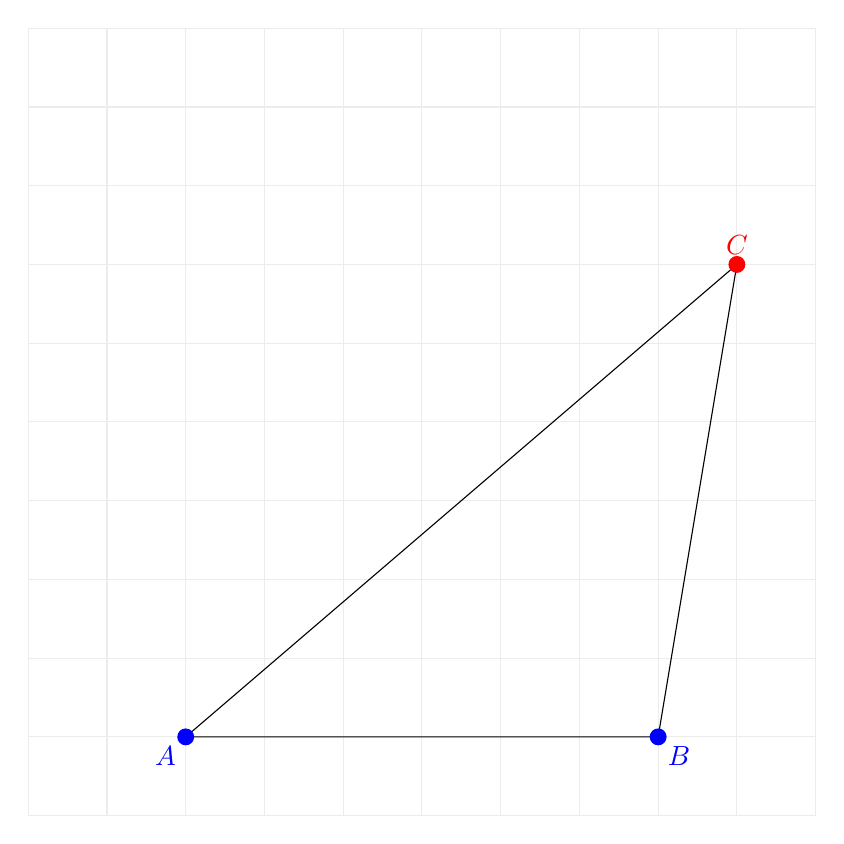
\begin{tikzpicture}[scale=1]
                \pgfmathsetmacro{\ax}{2}
                \pgfmathsetmacro{\ay}{1}
                \pgfmathsetmacro{\bx}{8}
                \pgfmathsetmacro{\by}{1}
                \pgfmathsetmacro{\cx}{9}
                \pgfmathsetmacro{\cy}{7}

                \draw[lightgray!30,thin] (0,0) grid (10,10);
		\draw[-] (\ax, \ay) -- (\bx, \by) -- (\cx, \cy) -- cycle;
		\filldraw[blue] (\ax, \ay) circle[radius=0.1] node[below left] {$A$};
		\filldraw[blue] (\bx, \by) circle[radius=0.1] node[below right] {$B$};
		\filldraw[red] (\cx, \cy) circle[radius=0.1] node[above] {$C$};

        \end{tikzpicture}
      \end{center}
 
\end{enumerate}

\newpage
\section*{Exercise 3}
Use SageMath to solve the following problems:
\begin{enumerate}[label=(\arabic*)]
	\item Find the roots of the following polynomial over $\mathbb Q$,
		over $\mathbb R$ and over $\mathbb C$:
		\[ p(x) = x^6+x^5-2x^4-3x^3-x^2+2x+2 \]
	\item Find the determinant, the trace and the characteristic polynomial
		   of the following matrix:
		\[A=
		\left(\begin{array}{rrrrr}
		2 & 3 & 0 & 1 & 2 \\
		1 & 0 & \frac{1}{2} & 1 & -1 \\
		0 & 0 & -1 & 0 & 0 \\
		0 & -1 & -1 & 0 & -1 \\
		-1 & -1 & -1 & -1 & 0
		\end{array}\right)
		\]
	\item Find the solutions of the linear system $A\mathbf x=\mathbf 0$, where
		$A$ is the matrix above and $\mathbf 0$ is the zero vector.
	\item Find the points of intersection of the circle of equation $x^2+y^2=4$
		   ad the ellipse of equation $\left(\frac{x}{2}\right)^2+(2y)^2=4$
	\item Plot the graph of the function $f(x)=\sqrt{1-x^6}$.
	\item Find the area between the $x$-axis and the grap of the function of
		   the previous point.
	\item Find the derivative, a primitive (integral) and the Taylor series
	      expansion up to order 4 of the function $h(x)=\log(1+x+x^2)$.
	\item Use Sage to get the Latex code for the objects you computed in
		the previous point.
	\item Find a solution for the differential equation with initial conditions
		   \[
			\begin{cases}g'(x)&=\frac{1}{3}g(x) - 7\\g(1)&=30\end{cases}
		   \]
	\item Draw a bar chart of the data set $[0,1,3,7,5,7,2,8,9,3]$, like the foll
	      following:
		\begin{center}
	      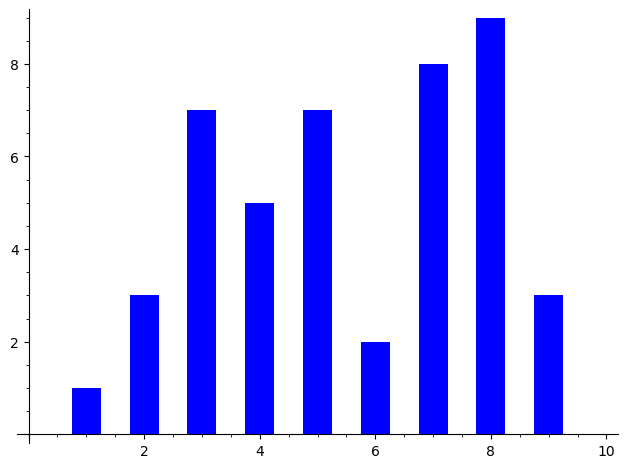
\includegraphics[scale=0.5]{bc.png}
	      \end{center}
\end{enumerate}

\newpage
\section*{Grading}

\vspace{0.3cm}
\textbf{Exercise 1 (5 points).}
\begin{itemize}
  \item A correct use of the \texttt{\textbackslash newtheorem} command is
        worth 2 out of 5 points.
  \item A correct use of the labelling and reference system is worth 2 points.
  \item Reproducing correctly the mathematical formulas is worth 1 point.
\end{itemize}

\vspace{0.3cm}
\textbf{Exercise 2 (5 points).}
\begin{itemize}
	\item Part (a) is worth 2 points: 1 point for having the letters
	      $M$, $N$ and $A$ in the correct position and the arrows
	      pointing between them and 1 point for the style of the arrows
	      and the labels $f$, $i$ and $\tilde f$ in the correct position.
	\item Part (b) is worth 3 points: 1 point for drawing a triangle, 1
	      point for the other decorative elements (colored dots, grid lines
	      and labels) and 1 point for having the point $C$ correctly set
	      as a macro so that it can be changed easily.
\end{itemize}

\vspace{0.3cm}
\textbf{Exercise 3 (10 points).}
\begin{itemize}
	\item Each of the 10 parts is worth 1 point.
\end{itemize}



\end{document}
